% This is based on "sig-alternate.tex" V1.9 April 2009
% This file should be compiled with V2.4 of "sig-alternate.cls" April 2009
%
\documentclass{report}

\usepackage[english]{babel}
\usepackage{graphicx}
\usepackage{tabularx}
\usepackage{subfigure}
\usepackage{enumitem}
\usepackage{url}
\usepackage[utf8]{inputenc}
\usepackage{textcomp} %for the degree symbol. yes. overkill
\usepackage{pgf}
\usepackage{tikz}
\usetikzlibrary{arrows,automata}
\usetikzlibrary{positioning}

\tikzset{
    state/.style={
           rectangle,
           rounded corners,
           draw=black, very thick,
           minimum height=2em,
           inner sep=2pt,
           text centered,
           },
}

\usepackage{color}
\definecolor{orange}{rgb}{1,0.5,0}
\definecolor{lightgray}{rgb}{.9,.9,.9}
\definecolor{java_keyword}{rgb}{0.37, 0.08, 0.25}
\definecolor{java_string}{rgb}{0.06, 0.10, 0.98}
\definecolor{java_comment}{rgb}{0.12, 0.38, 0.18}
\definecolor{java_doc}{rgb}{0.25,0.35,0.75}

% code listings
% code listings
\usepackage{listings}
\lstnewenvironment{Java}
  {\lstset{ language=Java,
	basicstyle=\scriptsize\ttfamily,
	backgroundcolor=\color{lightgray},
	keywordstyle=\color{java_keyword}\bfseries,
	stringstyle=\color{java_string},
	commentstyle=\color{java_comment},
	morecomment=[s][\color{java_doc}]{/**}{*/},
	tabsize=2,
	showtabs=false,
	extendedchars=true,
	showstringspaces=false,
	showspaces=false,
	breaklines=true,
	numbers=left,
	numberstyle=\tiny,
	numbersep=6pt,
	xleftmargin=3pt,
	xrightmargin=3pt,
	framexleftmargin=3pt,
	framexrightmargin=3pt,
	captionpos=b
  }
  }
  {}
\lstnewenvironment{XML}
  {\lstset{language=XML}}
  {}	

\lstdefinelanguage{XML}
{
  morestring=[b]",
  morestring=[s]{>}{<},
  morecomment=[s]{<?}{?>},
  stringstyle=\color{black},
  identifierstyle=\color{blue},
  keywordstyle=\color{cyan},
  morekeywords={xmlns,version,type}% list your attributes here
  basicstyle=\scriptsize\ttfamily,
	backgroundcolor=\color{lightgray},
	tabsize=2,
	showtabs=false,
	extendedchars=true,
	showstringspaces=false,
	showspaces=false,
	breaklines=true,
	numbers=left,
	numberstyle=\tiny,
	numbersep=6pt,
	xleftmargin=3pt,
	xrightmargin=3pt,
	framexleftmargin=3pt,
	framexrightmargin=3pt,
	captionpos=b
}

% Disable single lines at the start of a paragraph (Schusterjungen)

\clubpenalty = 10000

% Disable single lines at the end of a paragraph (Hurenkinder)

\widowpenalty = 10000
\displaywidowpenalty = 10000
 
% allows for colored, easy-to-find todos

\newcommand{\todo}[1]{\textsf{\textbf{\textcolor{orange}{[[#1]]}}}}

% consistent references: use these instead of \label and \ref

\newcommand{\lsec}[1]{\label{sec:#1}}
\newcommand{\lssec}[1]{\label{ssec:#1}}
\newcommand{\lfig}[1]{\label{fig:#1}}
\newcommand{\ltab}[1]{\label{tab:#1}}
\newcommand{\rsec}[1]{Section~\ref{sec:#1}}
\newcommand{\rssec}[1]{Section~\ref{ssec:#1}}
\newcommand{\rfig}[1]{Figure~\ref{fig:#1}}
\newcommand{\rtab}[1]{Table~\ref{tab:#1}}
\newcommand{\rlst}[1]{Listing~\ref{#1}}

% General information

\title{Distributed Systems -- Final Project}

% Use the \alignauthor commands to handle the names
% and affiliations for an 'aesthetic maximum' of six authors.

\numberofauthors{3} %  in this sample file, there are a *total*
% of EIGHT authors. SIX appear on the 'first-page' (for formatting
% reasons) and the remaining two appear in the \additionalauthors section.
%
\author{
% You can go ahead and credit any number of authors here,
% e.g. one 'row of three' or two rows (consisting of one row of three
% and a second row of one, two or three).
%
% The command \alignauthor (no curly braces needed) should
% precede each author name, affiliation/snail-mail address and
% e-mail address. Additionally, tag each line of
% affiliation/address with \affaddr, and tag the
% e-mail address with \email.
%
% 1st. author
\alignauthor Lukas Häfliger\\
	\affaddr{ETH ID 11-916-376}\\
	\email{haelukas@student.ethz.ch}
% 2nd. author
\alignauthor Alexandra Maximova\\
 	\affaddr{ETH ID 09-913-534}\\
 	\email{amaximov@student.ethz.ch}
%% 3rd. author
 	\alignauthor Thomas Müller\\
 	\affaddr{ETH ID 11-946-936}\\
 	\email{muelltho@student.ethz.ch} 
\and  % use '\and' if you need 'another row' of author names	
%% 4th. author
\alignauthor Christian Vonrüti\\
 	\affaddr{ETH ID 11-930-914}\\
 	\email{cvonruet@student.ethz.ch} 
%% 5th. author
\alignauthor Alexander Viand\\
	\affaddr{ETH ID 09-940-131}\\
	\email{vianda@student.ethz.ch}
%% 6th. author
\alignauthor Marko Živković\\
	\affaddr{ETH ID 10-921-211}\\
	\email{markoz@student.ethz.ch}
}


\begin{document}

\maketitle

\begin{abstract}
We present a cross-platform game called Tronium that allows up to eight players (who can be using different platforms) to play together via local network, 
or alternatively allows single-player matches against AI opponents. 

Tronium is inspired by the "light cycle" scene from the 1982 film "Tron" and is implemented using the  Unity\textregistered   \ Engine, which is a high-level framework for game development.
The game supports Windows on x86/x86\_64 and Android\texttrademark \ 
with potential for easy ports to others platforms thanks to the cross platform capabilities of the Unity engine.

\end{abstract}

\section{Introduction}

We were inspired to create this game after playing Armagetron Advanced, an open source game that is itself inspired by the light cycle scene from "Tron". 
In Section 2 we will look at Armagetron Advanced and other games inspired by Tron, as well as similar games available on mobile platforms.
In Section 3, we will explain the gameplay and game mechanics that we decided to implement with Tronium, and in  Section 4 we will introduce Unity with a focus on its networking concepts. In Section 5 we will show how we use these concepts in our game. 
In Section 6 we show our implementation of collision detection and prediction, ensuring reasonable behaviour in case of network delays that are "long" in comparison to the high in-game speeds.
In Section 7 we introduce the AI that we use in the single-player mode as well as our own extension to the game,  randomly roaming obstacles.
In the last section, we will give our conclusions on our game and working both with Unity as well as with a larger group.

 
\section{Existing games}

Armagetron Advanced\cite{AA} is one of two open source projects that try to recreate the light cycle scene, the other being GLTron\cite{GLT} by Andreas Umbach\cite{Umbach}.
GLTron is a more faithful reproduction both visually as well in terms of game mechanics of the original light cycle scene from the 1982 film while Armagetron Advanced is further removed from the original visually and offers a wide variety of gamemodes that go far beyond what is seen in the film as well as heavy customization, with parameters like base speed, arena size, number of players, etc.
We were aiming more at recreating the enjoyment of playing Armagetron Advanced rather than being faithful to the original scene.
Since the scope of this project was somewhat limited, we do not offer the extensive options and choice of game mode that Armagetron Advanced does, 
but rather focused on implementing the 'core' game mode with fixed parameters. Visually, we were inspired by the aesthetics of the 2010 film "Tron Legacy" rather than by the original film or the existing games

Armagetron Advanced offers local (split-screen), local network and internet multiplayer.
Armagetron Advanced itself is available for Windows, Linux and Mac OS but does not have an Android (or other mobile platform) port.
 There exists an android game called Androgetron\cite{Andro} developed by a member of the Armagetron Advanced community,however this is a much simplified clone without networked multiplayer.
  On the official Google Play\texttrademark Store there are a few more games\cite{GP1}\cite{GP2}\cite{GP3} that are essentially identical to Androgetron and seem to be all based on an android port of GLTron. They also do not offer any kind of non-split-screen multiplayer.

Split screen is a viable option on a full size laptop or desktop monitor, however it feels very cramped even on larger tablets and is essentially unusable on smartphones.
Our goal was therefore to implement a true (networked) multiplayer experience on mobile devices.
Instead of trying to adapt the large and complex code base of Armagetron Advanced (or GLTron), we decided to implement a version of the game with smaller scope from scratch.
We decided to use Unity, a high level game engine and Integrated Development Engine (IDE) (which will be discussed in Section 4) to implement the following game mechanics:

\begin{figure}
 	 	    \includegraphics[height=6cm]{tron_four}
 	  
 	 	\caption{The main game... << weird wall >> }
 \end{figure}
 
 \section{Tronium mechanics }
We simplified the complex settings and mechanics from Armagetron Advanced to a single game mode, with fixed speed, arena size, etc.
We did, however, also extend the game to new concepts not present in any of the other versions. Specifically, we introduced collectible "powerups" and moving obstacles that roam the arena.

The game takes place in a (square) arena, in which the players drive with their "light cycles" (from now on simply bike).
The bike moves constantly and can only be turned 90\textdegree left or right.
Each bike leaves a solid trail (wall), and collisions with either the sides of the arena, your own wall or another player's wall will result in your death.
The aim is to avoid collisions and to be the last player alive.
Being close to another wall increases your speed, allowing you to e.g. overtake and 'box in' another player.
There are also two different types of powerups that spawn randomly throughout the arena. 
They grant a temporary speed bonus or temporary invincibility (allowing the player to go through walls).
There are also additional obstacles in form of large cubes that slowly 'roll' around the arena. Collisions with these obstacles also results in the player's death. 

For single-player games, there are AI opponents which will take the role of other players (i.e. drive bikes as well).
The AI and the roaming obstacles will be described in more detail in Section 7.


\begin{figure}
\centering
\subfigure[client] {
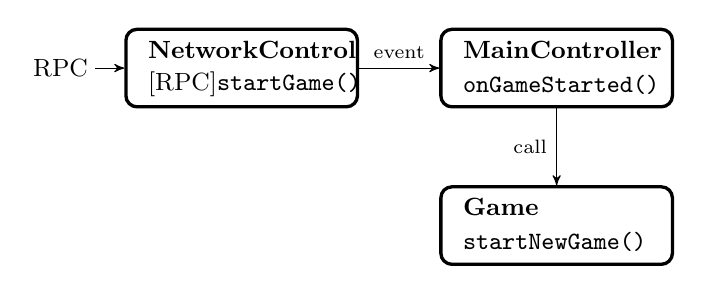
\begin{tikzpicture}[->,>=stealth']

 % First node
 % Use previously defined 'state' as layout (see above)
 % use tabular for content to get columns/rows
 % parbox to limit width of the listing
 \node[state,draw=none] (RPC) 
 {\small{RPC}};

 % Next node: NetworkControl
 \node[state,       % layout (defined above)
 node distance=2.3cm,     % distance to RPC
 text width=2.8cm,        % max text width
 right of=RPC](NC)       % Position is to the right of RPC (NC)
 {%                     % posistion relative to the center of the 'box'
 \begin{tabular}{l}     % content
  \small{\textbf{NetworkControl}}\\
  \parbox{2.6cm}{\small{[RPC]\texttt{startGame()}}}
 \end{tabular}
 };

 % STATE MainController
 \node[state,
 right of=NC,
 node distance=4cm,
 text width=2.8cm] (MC) 
 {%
 \begin{tabular}{l}
  \small{\textbf{MainController}}\\
  \parbox{2.6cm}{\small{\texttt{onGameStarted()}}}
 \end{tabular}
 };

 % STATE Game
 \node[state,
 below of=MC,
 node distance=2cm,text width=2.8cm] (Game) 
 {%
 \begin{tabular}{l}
  \small{\textbf{Game}}\\
  \parbox{2.6cm}{\small{\texttt{startNewGame()}}}
 \end{tabular}
 };

 % draw the paths and and print some Text below/above the graph
 \path (RPC) edge node {} (NC)
       (NC)  edge node [anchor=south]{\scriptsize{event}}  (MC)
       (MC)  edge node[anchor=east] {\scriptsize{call}} (Game)
 ;
\end{tikzpicture}
}

\hfill
\subfigure[server]{

\begin{tikzpicture}[->,>=stealth']

 % First node
 % Use previously defined 'state' as layout (see above)
 % use tabular for content to get columns/rows
 % parbox to limit width of the listing
 \node[state,draw=none] (GUI) 
 {\small{GUI}};

 % Next node: MainController
 \node[state,       % layout (defined above)
 node distance=2.3cm,     % distance to RPC
 text width=2.7cm,        % max text width
 right of=GUI](MC)       % Position is to the right of RPC (NC)
 {%                     % posistion relative to the center of the 'box'
 \begin{tabular}{l}     % content
  \small{\textbf{MainController}}\\
  \parbox{2.5cm}{\small{\texttt{startNetwokGame()}}}
 \end{tabular}
 };

 % STATE NetworkControl
 \node[state,
 right of=MC,
 node distance=3.6cm,
 text width=3.1cm] (NC) 
 {%
 \begin{tabular}{l}
  \small{\textbf{NetworkControl}}\\
  \parbox{2.9cm}{\small{\texttt{broadcastNewGame()}}
  				\small{[RPC]\texttt{startNewGame()}}
 	}
 \end{tabular}
 };

 % STATE SameAsClient
 \node[state,draw=none,
 below of=NC,
 node distance=1.3cm,
 text width=2.2cm] (SAC) 
 {%
 \begin{tabular}{l}
  \parbox{2.5cm}{Same as client}
 \end{tabular}
 };

 % draw the paths and and print some Text below/above the graph
 \path (RPC) edge node {} (MC)
       (MC)  edge node [anchor=south]{\scriptsize{call}}  (NC)
       (NC)  edge [loop right, min distance=10mm,in=-7,out=7,looseness=1] node[anchor=east] {\small{RPC}} (NC)
       (NC) edge [bend left=40] (SAC.east)
 ;
\end{tikzpicture}
}
\caption{Control flow diagrams}
\end{figure}

\begin{figure}
\centering
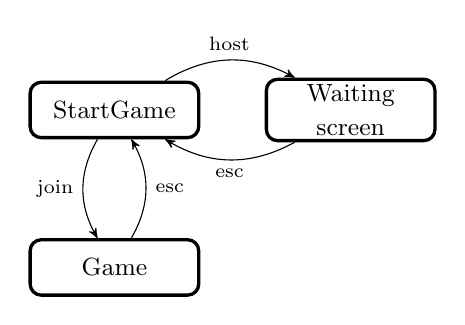
\begin{tikzpicture}[->,>=stealth']

 % First node
 % Use previously defined 'state' as layout (see above)
 % use tabular for content to get columns/rows
 % parbox to limit width of the listing
 \node[state,text width=2cm] (SG) 
 {\small{StartGame}};

 % Next node: WS (no idea what these letters should mean)
 \node[state,       % layout (defined above)
 node distance=3cm,     % distance to SG
 text width=2cm,        % max text width
 right of=SG](WS)       % Position is to the right of SG
 {\small{Waiting screen}};

 % STATE Game
 \node[state,
 below of=SG,
 node distance=2cm,
 text width=2cm] (Game) 
 {\small{Game}};

 % draw the paths and and print some Text below/above the graph
 \path (SG) edge [bend left] node [anchor=south] {\scriptsize{host}} (WS)
 (WS) edge [bend left] node [anchor=north] {\scriptsize{esc}} (SG)
       (SG)  edge [bend right] node [anchor=east]{\scriptsize{join}}  (Game)
       (Game) edge [bend right] node [anchor=west] {\scriptsize{esc}} (SG)
 ;
\end{tikzpicture}
\caption{Control flow}
\end{figure}

\section{Unity}
Unity\textregistered, which is developed by Unity Technologies, is a high level game development framework or engine. Our project specifically uses the commercial version of Unity called Unity\textregistered Pro. Unity offers an editor  <<FIGURE>> that allows manipulation of 3D environments, game assets and live debugging.
Unity is based on Mono (an open source .NET-compatible framework) and allows development in \\ JavaScript, Boo or C\#. 
We chose to use C\# because of its similarities to Java and Unity's integration with the extremely powerful Visual Studio IDE.
Unity supports a large number of platforms, including x86/x86\_64 (Windows, Mac OS and Linux), Android, iOS and Windows Phone 8, with a generally very small required effort for porting between platforms.
The support for native x86 versions greatly reduced the time needed for testing and debugging during development.

Unity's core concept is that of a "scene" which is an abstraction of a 3D space that contains "GameObject"s.
\\ "GameObjects" are containers that contain "Component"s (which can also be GameObjects, allowing for nesting).
All "GameObject"s have a basic "transform" "component" which contains information about position, rotation and velocity of the "GameObject". There are many other types of "Component"s, including "Lights", "Cameras" and "Materials" as well as Scripts.

Unity offers two very different methods for networking.
A high-level "synchronization" feature as well as comparatively "low level"  Remote Procedure Calls (RPC).
Both require a GO to have a "NetworkView" component which makes them visible to the network in Unity.

Synchronization allows for high-frequency, low-cost updates  of GOs. It can however only be used to synchronize certain properties of the GO, e.g. the transform (pos,rot,vel) component.

RPC on the other hand, is intended to be used for less frequent and less time-sensitive communication and is very similar to RPC implementations in other frameworks.

\section{Tronium networking}
Tronium combines (as do most Unity applications) both methods, using Synchronization for player and wall positions (or more correctly player and wall "transforms"), as well as RPC for communicating gamestate changes.

In terms of networked multiplayer, most games can be classified into either an authoritative or non-authoritative server style.

With a non-authoritative server, clients will do their own calculations locally and based on those will report e.g. their player's new position and events like the player's death to the server (and potentially other players). This is in contrast to an authoritative server, where the client is mostly reduced to relaying the users input to the server which in turn does the necessary calculations and sends back information about   e.g. the player's position and liveness back to the clients.

Authoritative servers have the advantage of preventing many common forms of cheating that involve running modified client code, however they also require a more powerful machine as server and result in additional latency.

Since our game is quite fast paced and supposed to run on relatively low-power mobile devices and will most likely not be subject to complicated cheating attempts, we feel that non-authoritative server was the best fit for our application.


Updates regarding the movement of the player and the creation of new walls in a player's trail are handled by the player instance and are communicated using Unity's "state synchronization" system. 
The system offers two options for data transfer. One is a unity-specific reliable data protocol that uses delta compression (i.e. sending only the information that has changed) and ensures in-order delivery. The other is unreliable transmission via UDP.
Since in a racing game low latency is more important than in order-delivery, we use the UDP transmission mode. All clients will locally extrapolate (based on last known speed) the position of other players' bikes. In Section 6 we will explain how we deal with network delay when calculating collisions and player deaths to ensure that players will never be 'retroactively' killed because of information that arrives late.

Spawning of new GameObjects (e.g. walls) is done via Unity's Network.Instantiate method, which automatically creates the same object on all clients.

Less frequent updates like e.g. player deaths and game start/end are sent via RPC.

Since unity does not have a high-level concept representing the current application instance in its entirety, every script has to be attached to a GameObject and each instance (client?) will execute the same code for a given GameObject. 
Since our server instance will also be acting as a player/client instance, this model works well with our application design.

Checks like "Network.isMine()" or "Network.isServer()" allow to test wether the current GameObject (or more specifically its NetworkView) is owned by the current instance and whether we are acting as the server, respectively. 

Their is an "empty" (i.e. code-only) GameObject that contains the "MainController" which is responsible for updating the GUI and communicating (locally) state changes between the Game and the NetworkController.

The NetworkController causes events (via delegates) to be triggered in the MainController, which will then in turn call methods of the NetworkController or GameController.
The NetworkController handles all RPC. A received RPC will result in an event being triggered in MainController.
The MainController calls (non-RPC) functions of the NetworkController which will then in turn send out RPC Calls  to the network.
In our implementation RPC's will also be sent to the sender, ensuring that all clients make the same state transitions.
See <<FIGURE>> for examples of (simplified) state transitions involved with starting a new game via network.


\section{Collision detection}
If (drove into wall) \{
	players the Died 
	\}
	<< << marko >> >>

\section{Computer controlled opponents}
In local singleplayer, there are computer controlled bikes that follow a simple pattern. 
Whenever a computer controlled bike predicts a wall collision (using the same code as above), it will (with high probability) do a "saving" turn (with equal probability for left and right turns). To ensure that they cannot survive forever, they are only allowed to do these "saving" turns every second frame.

To avoid making the AI too predictable, there is also a chance that they will randomly (again, left right being equally likely) turn even if they do not detect any walls.

This results in a very simple AI, however since the game is mostly about reflexes this unpredictable AI works well enough to make the single-player mode enjoyable.

As more relentless enemies pose randomly moving cubes. Such a cube moves by rotating over one of its edges touching the ground as depicted by << << image >> >>. To achieve the movement as illustrated in the aforementioned image---assuming the pivot were in the center---the cube must be translated in two directions and rotated simultaneously over time. However, if we choose to rotate around the blue axis (which represents time in the image), none of this is necessary. Fortunately, Unity provides a \prog{RotateAround()} method to do just that. Our implementation can rotate only over one of the cubes edges. To allow movement in any diretion, we simply rotate the cube around it's center before initiating the movement. This works because the cube's sides are uniform: a 90° rotation is, as far as the viewer is concerned, invisible. This axis is specified by two vectors, an origin relative to the cube's center: \{x: -.5, y: -.5, z: -.5 \} and another vector to indicate the direction: \{x: 0, y: 0, z: 1\}. Unity cube primites have an edge length of 1, which produces $-0.5$ used in the coordinates. However, \prog{RotateAround()} expects the axis to be in world coordinates, for this we transform both the origin and the direction out of our local coordinate system again leveraging Unity's built-in methods. Now that all pieces are in place, for the animation.  our rotation axis Due to time constraints, cubes are allowed to move through any geometry. As an improvement, one might consider to have cubes tear down pieces of walls they come into contact.


\section{Conclusion}
 Working in a larger group was an interesting change and while our intra team communication was very good there were considerable efficiency losses when e.g. bug fixes for one component affected code that was concurrently being refactored.

 We feel that we accomplished our goal of creating an enjoyable  networked multiplayer version of a "Tron-like game" for mobile devices. Unity allowed us to very quickly create the visual aspects of the game and allowed us to focus on the distributed networking component of the game.

An obvious and straight forward next step would be allowing the  player to customize the parameters of the game. Another interesting extension would be internet multiplayer, however additional work for NAT and higher latencies might be necessary.

\balancecolumns % GM June 2007

% The following two commands are all you need in the
% initial runs of your .tex file to
% produce the bibliography for the citations in your paper.
\bibliographystyle{abbrv}
\bibliography{report}  % sigproc.bib is the name of the Bibliography in this case
% You must have a proper ".bib" file


\end{document}
